% ------------------ DOCUMENT SETUP ------------------ 
% The document class defines the document type (report) and sets the font size (12pt)
\documentclass[12pt]{report}
\author{Juan Jesús Torres Solano}


% ------------------ PACKAGES ------------------ 
% Packages add extra commands and features to your LaTeX document. 
% In here, some of the most common packages for a thesis document have been added 


\usepackage{float}% LaTeX's float package
\usepackage{color}% LaTeX's color package
\usepackage[spanish]{babel}%lenguaje de indicadortes
\usepackage{amsmath}% LaTeX's main math package
\usepackage[format=plain,font=footnotesize,labelfont=bf]{caption}% LaTeX's Caption and subcaption packages
\usepackage{subcaption}
\usepackage{graphicx}% The graphicx package provides graphics support for adding pictures.
\usepackage{longtable}% Longtable allows you to write tables that continue to the next page.
\usepackage[a4paper, lmargin=2.5cm, rmargin=2.5cm, tmargin=2.5cm, bmargin=2.5cm]{geometry}% The geometry packages defines the page layout (page dimensions, margins, etc)
\usepackage[sfdefault]{arimo}% Defines the Font of the document, e.g. Arimo font (Check Fonts here: https://tug.org/FontCatalogue/)
\usepackage[T1]{fontenc}% Font encoding
\usepackage[utf8]{inputenc}% This package allows the user to specify the input encoding
\usepackage{emptypage}% This package allows you to add empty pages
\usepackage{import}% Allows inputs to be imported from a directory
\usepackage{tocloft}% Provides control over the typography of the Table of Contents, List of Figures and List of Tables
\usepackage{setspace}% The setspace package controls the line spacing properties.
\usepackage{titlesec}% Allows the customization of Latex's title styles
\usepackage{titletoc}% Allows the customization of Latex's table of contents title styles
\usepackage{etoolbox}% The package provides functions that offer alternative ways of implementing some LATEX kernel commands
\usepackage{fancyhdr} % Provides extensive facilities for constructing and controlling headers and footers
% Typographical extensions, namely character protrusion, font expansion, adjustment 
%of interword spacing and additional kerning
\usepackage{microtype}
\usepackage[colorlinks=true,linkcolor=black,urlcolor=black,citecolor=black]{hyperref}% Manages hyperlinks 
\usepackage{bookmark}% Generates PDF bookmarks
\usepackage[table,xcdraw]{xcolor}% Add color to Tables
\usepackage{gensymb}% Use these two packages together -- they define symbols
\usepackage{textcomp}%  for e.g. units that you can use in both text and math mode.
\usepackage[acronym]{glossaries}% Acronym Package
\usepackage{matlab-prettifier}% Package for Matlab code
\usepackage{relsize}% Change font size
\usepackage{blindtext}% Blindtext (only for template) texto muestra
\usepackage[table,xcdraw]{xcolor}
\usepackage{colortbl}

\usepackage{listings}


% Controls how many subsections the document can take
%  and how many of those will get put into the contents pages.
\setcounter{secnumdepth}{3}
\setcounter{tocdepth}{3}

% Line Spacing
\setstretch{1}


% Places a dot after Chapter/Section/Subsection number in Table of Contents
\renewcommand{\cftchapaftersnum}{.}
\renewcommand{\cftsecaftersnum}{.}
\renewcommand{\cftsubsecaftersnum}{.}

%  Customize Dot spacing in Table of Contents/List of Figures/Tables
\renewcommand{\cftdotsep}{0.3}


% Line Break Properties
\tolerance=1
\emergencystretch=\maxdimen
\hyphenpenalty=10000
\hbadness=10000


% Formatting Table of Contents/Lists titles
\renewcommand{\contentsname}{\bfseries\LARGE{INDICE}}
\renewcommand{\listfigurename}{\bfseries\LARGE{LISTA DE FIGURAS}}

% Signature Line for the declaration
\newbox\namebox
\newdimen\signboxdim

\def\signature#1{%
    \setbox\namebox=\hbox{#1}
    \signboxdim=\dimexpr(\wd\namebox+3cm)
    \parbox[t]{\signboxdim}{%
        \centering
            \hrulefill\\    % for a line
            #1
        \par}%
    }

% Title Formatting customization
\titleformat{\chapter}{\normalfont\bfseries\LARGE}{\thechapter.}{1em}{\MakeUppercase}

\titleformat{\section}{\normalfont\bfseries\large}{\thesection.}{1em}{\MakeUppercase}
\titlespacing*{\section} {0pt} {0pt} {15pt} % left, before, after

\titleformat{\subsection}{\normalfont\bfseries\large}{\thesubsection.}{1em}{}
\titlespacing*{\subsection} {0pt} {10pt} {10pt}

\titleformat{\subsubsection}{\normalfont\bfseries\large}{\thesubsubsection.}{1em}{}
\titlespacing*{\subsubsection} {0pt} {10pt} {10pt}


% HEADER AND FOOTER
\pagestyle{fancy}  % Set Page Style (Header and Footer Style)
\fancyhf{}  % Clears the header and footer (from the default info)

% Header
\renewcommand{\headrulewidth}{0pt}  % Removes the default Horizontal Line in Header
% Optional Headers
%\fancyhead[L]{}
%\fancyhead[R]{2022/2023}

% Footer
\fancyfoot[C]{\thepage} % Page Number

% Change figure numbering per section
\numberwithin{figure}{chapter}


%  -------------------------------------------------
%  --------- The document starts from here --------- 
%  -------------------------------------------------

\begin{document}


% ------------------  TITLE PAGE -------------------
\begin{titlepage}
\begin{center}
    % UCL IMAGE
    \vspace*{-2cm}
    \makebox[\textwidth]{
\includegraphics[width=0.7\paperwidth]{Images/UANL}}
    
    \vspace{1.5cm}
    
    % Title
    %{\relscale{1.19}{A thesis submitted in partial fulfilment of the requirements for the degree of Master of Science (MSc) in}}

    \vspace{1cm}
    {\relscale{1.15}\textbf{Maestría en Ciencia de Datos\\}}
    \vspace{0.3cm}
    {\relscale{1.15}\textbf{Universidad Autónoma de Nuevo León\\}}
    \vspace{2.4cm}
    
    {\relscale{2}{Tarea 1 - Análisis estadístico de comentarios del primer debate presidencial}}\\
    %\vspace{0.1cm}
    Por\\
    %\vspace{0.1cm}
    Juan Jesús Torres Solano\\
    \vspace{0.9cm}
    {\begin{singlespace}Profesor: José Alberto Benavides Vázquez \\
    %Second Supervisor: \\
	\end{singlespace}}
\end{center}
%{\raggedleft\vfill{\begin{singlespace}
%     Department of Medical Physics\\
%  and Biomedical Engineering\\
%\end{singlespace}
% UNIVERSITY COLLEGE LONDON\\
% \begin{singlespace}
% Date of submission: \today\\
% Word count: WORD COUNT\\
% \end{singlespace}
%}\par
%}
\end{titlepage}

% ----------------------  DECLARATION -----------------------
%\newpage
%\chapter*{Declaration} % the Asterix (*) indicates that this section will be added to the table of contents but no number will be present beside it.
%\addcontentsline{toc}{chapter}{Declaration}
%I, YOUR NAME confirm that the work presented in this report is my own. Where information has been derived from other sources, I confirm that this has been indicated in the report.
%\vspace*{3cm}

%\noindent\signature{YOUR NAME}
%\newpage
% ----------------------  ABSTRACT -----------------------
%\newpage
%\chapter*{Abstract} % the Asterix (*) indicates that this %section will be added to the table of contents but no %number will be present beside it.
%\addcontentsline{toc}{chapter}{Abstract}
%\blindtext

% -----------------  ACKNOWLEDGEMENTS  -------------------
%\newpage
%\chapter*{Acknowledgements}
%\addcontentsline{toc}{chapter}{Acknowledgement}
%\blindtext
%\newpage
% -----------------  ACRONYMS  -------------------
%\newpage
%\chapter*{Acronyms}
%\addcontentsline{toc}{chapter}{Acronyms}
%\printglossary[type=\acronymtype,nonumberlist,nopostdot]
%\newpage
% ------------------  TABLE OF CONTENTS --------------------
\tableofcontents 
% -------------------  LIST OF FIGURES --------------------
\newpage 
{\let\oldnumberline\numberline       % Uncomment to add the word 'Figure' to figure number in List of Figures
\renewcommand{\numberline}{\figurename~\oldnumberline}  
\listoffigures}
\addcontentsline{toc}{chapter}{ÍNDICE DE FIGURAS} % Add List of figures into contents without any numeration 
% -------------------  INTRODUCTION  ---------------------
\chapter{Introducción}

Los comentarios en videos en vivo son parte importante de la respuesta de la audiencia y se entiende que estos comentarios este cargados de palabras emotivas o que representen los sentimientos que las personas intentan comunicar al resto de espectadores, incluso a los mismos creadores del contenido o participantes de la transmisión en vivo, por lo que es de esperar que estos se expresen de forma positiva o negativa, de igual forma estos comentarios pueden ser poco objetivos, claramente objetivos o muy subjetivos\cite{steven2024}.\\

El análisis de sentimientos implica el procesamiento del lenguaje natural de modo que se logre identificar información subjetiva de un texto en particular, en esta tarea buscamos identificar el sentimiento subjetivo expresado por los usuarios que dejaron un comentario en la transmisión en vivo del primer debate presidencial \cite{quiroga2016}\cite{steven2024}.\\

\section{Objetivos}
El objetivo de este trabajo es identificar el sentimiento expresado por los usuarios en los comentarios del debate, teniendo en cuenta los votos que recibieron los comentarios y el sentimiento presente en aquellos mas votados, al igual que la respuesta general de los sentimientos de la audiencia; y por lo tanto  se requiere establecer su identificación, distribución y cuantificación:\\

\begin{enumerate}
	\item Identificar y cuantificar la polaridad de los comentarios que la audiencia dejo en el video del debate.\\
	
	\item Identificar y cuantificar el nivel de objetividad y subjetividad de los comentarios en el video.\\
\end{enumerate}


\chapter{Análisis de sentimiento}

Para el análisis de sentimiento se empleo la librería de TexBlod, la cual tiene como objetivo ofrecer un entorno familiar, cómodo e intuitivo empleado Python, esta librería nos permite emplear su modelos entrenados para clasificar el sentimiento subjetivo reflejado en las palabras empleadas en los comentarios, así como la objetividad de los mismos \cite{steven2024}.\\

A partir de esta clasificación obtendremos una asignación de peso para cada comentario, el cual esta expresado como "Polaridad" este valor representa sentimientos positivos o negativos, haciendo referencia al concepto de polaridad \cite{quiroga2016}, la escala esta representada de la siguiente manera, donde $ c = comentario$ :\\

\begin{itemize}
	\item Se consideran con polaridad muy negativa 
	\begin{itemize}
		\item $ -1\leq C < 0 $
	\end{itemize}
	\item Se consideran con polaridad neutral 
	\begin{itemize}
		\item $ C = 0 $
	\end{itemize}
		\item Se consideran con polaridad muy positiva 
	\begin{itemize}
		\item $0< C  \leq 1 $
	\end{itemize}
\end{itemize}

Mientras que la objetividad presenta dos limites donde un comentario de puede interpretar como objetivo, es decir presenta una estructura la cual contiene información sin incluir opiniones ni sentimientos, o subjetivo expresando su punto de vista, opinión personal o sentimientos, se clasifica mediante la siguiente escala, donde $ c = comentario$: \\

\begin{itemize}
	\item Se consideran objetivo
	\begin{itemize}
		\item $ C \geq 0 $
	\end{itemize}
	\item Se consideran subjetivo
	\begin{itemize}
		\item $ C \leq 1 $
	\end{itemize}
\end{itemize}

\chapter{Resultados}

A partir de los resultados obtenidos mediante el análisis de sentimientos, podemos observar la distribución de frecuencias de los pesos asignados a la objetividad y polaridad de cada comentario, a partir de esta distribución se observa lo siguiente (ver fig \ref{fig:dpys}).\\

Para una mejor visualización de la distribución las frecuencias esta se representa empleando escala logarítmica.\\
 
\begin{figure}[!h]
	\centering
	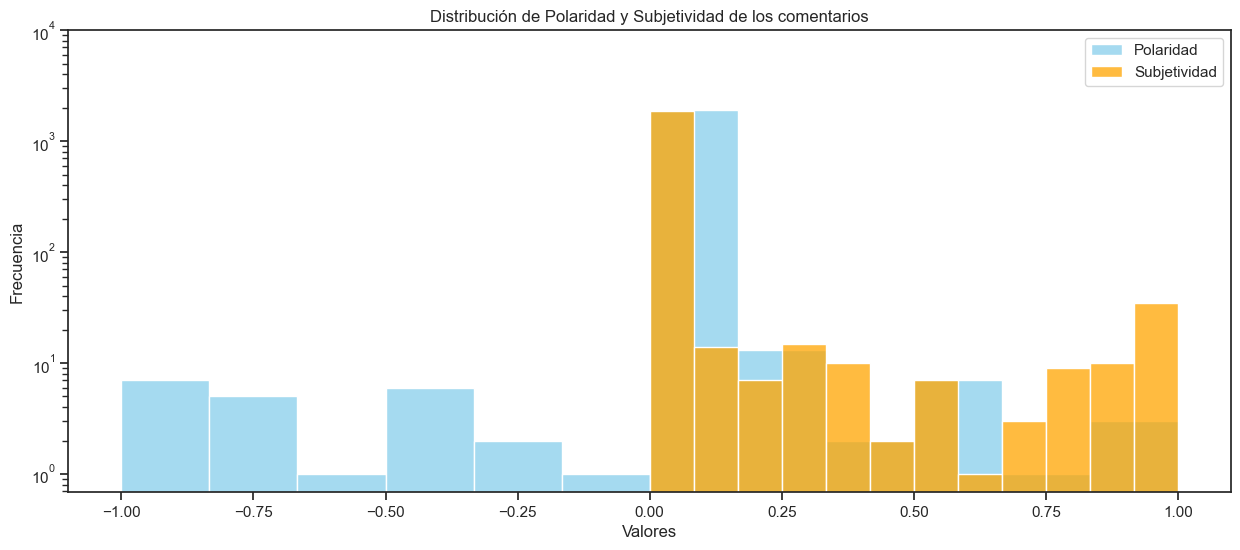
\includegraphics[width=16cm]{../Datos/polaridadYsubjetividad}
	\caption[Distribución de polaridad y subjetividad]{Distribución de la polaridad y subjetividad de los comentarios del primer debata presidencial.}
	\label{fig:dpys}
\end{figure}

Podemos observar que la distribución de polaridad se concentra en la porción central, es decir se identifica predominantemente comentarios con mayor tendencia de polaridad neutral, sin embargo se observa un numero mayor de comentario con tendencia negativa que aquellos con tendencia positiva, a partir de este comportamiento podemos concluir que los comentarios de los usuarios son mayormente neutrales (ver fig \ref{fig:dpys}).\\

La subjetividad por otro lado muestra coherencia en la distribución con respecto a la polaridad, se identifica un numero alto de comentarios objetivos mientras que la distribución de los comentarios subjetivos presenta una menor distribución, sin embargo, en conjunto es notorio un aumento de la subjetividad dentro del rango próximo al valor de 1 (ver fig \ref{fig:dpys}).\\
\clearpage
 
\begin{figure}[!h]
	\centering
	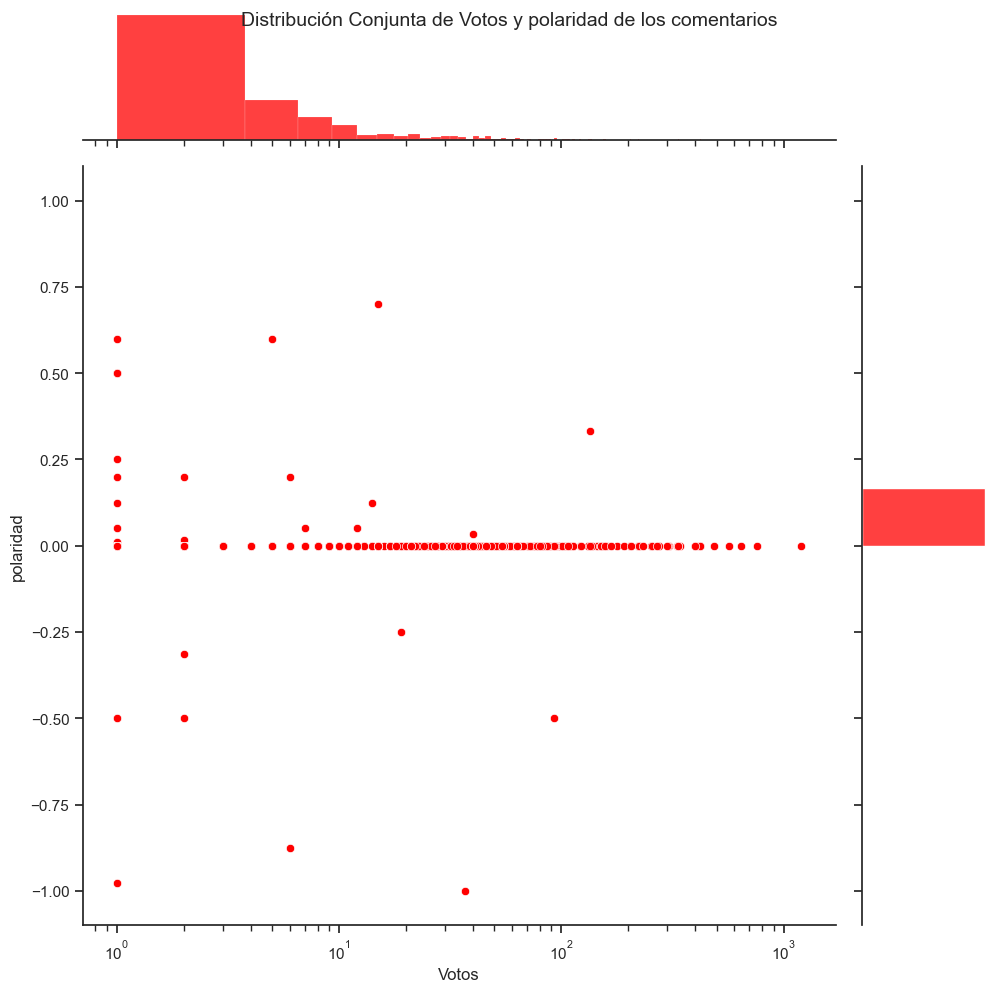
\includegraphics[width=16cm]{../Datos/DisVotosPolaridad}
	\caption[Distribución de frecuencia de voto y su polaridad]{Distribución de votos y la polaridad asociada con el interés y aprobación del publico.}
	\label{fig:dvp}
\end{figure}

Al revisar la distribución de los comentarios mas votados y su correspondiente valor de polaridad podemos notar una polaridad dispersa en comentarios con un menor numero de votos, pudiendo significar esto la poca aprobación de comentarios demasiado negativos o positivos.\\

\begin{figure}[!h]
	\centering
	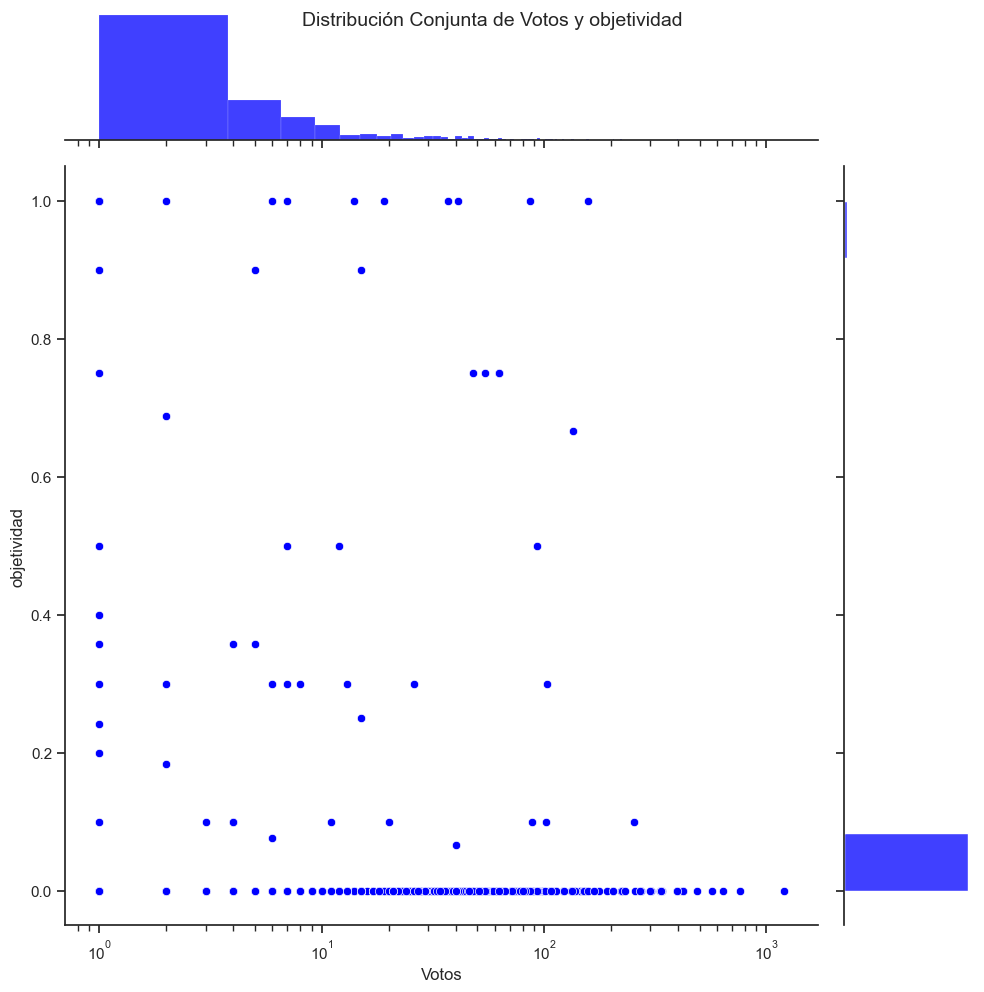
\includegraphics[width=16cm]{../Datos/DisVotosObjetividad}
	\caption[Distribución de frecuencia de voto y objetividad]{Distribución de la frecuencia de los votos y la objetividad de los comentarios}
	\label{fig:dvo}
\end{figure}

En cuanto a la distribución conjunta de frecuencias de votos y objetividad, podemos destacar la los comentarios con menor numero de votos presentan subjetividad en el texto, sin embargo la distribución de comentarios con algún grado de subjetividad presentan una distribución dentro del rango de 0 a 300 votos, encontrándose lejos del top 20 de comentarios mas votados. 

\chapter{Conclusiones}

Se puede concluir que los comentarios objetivos y neutrales son aquellos mas votados por el publico que observo y participo en el chat del debate.\\ 

De igual forma se observa un apoyo menos concentrado en aquellos comentarios que presentan algún sesgo de preferencia o repudio sobre algún candidato, tema, proceso, etc...\\

Estas observaciones 
 
% -------------------  MATERIALS AND METHODS  ---------------------
%\chapter{Fuente y descripción de los datos}

\section{método de recopilación}


\chapter{Metodología} 
% -------------------  RESULTS  ---------------------
%\blindtext 
% -------------------  DISCUSSION  ---------------------
%\chapter{Discusión}   
% -------------------  CONCLUSION AND FUTURE OUTLOOK  ---------------------
%\section{Conclusion}
\blindtext \\

\section{Future Outlook}
\blindtext
\newpage
\bibliographystyle{elsarticle-num.bst}
\bibliography{References}
\addcontentsline{toc}{chapter}{References} % Adds References Section to Table of Contents
% -------------------  Appendix  ---------------------
%\chapter*{Appendix}
\end{document}
%  -------------------------------------------------
%  --------- The document ends from here ----------- 
%  -------------------------------------------------